\documentclass[
    12pt,
    openright, 
    oneside,
    %twoside, %TCC: Se seu texto tem mais de 100 páginas, descomente esta linha e comente a anterior
    a4paper,
    french,
    english,
    brazil
    ]{facom-ufu-abntex2}

\usepackage[disable]{todonotes}
%\usepackage[colorinlistoftodos]{todonotes}	%use a linha anterior para esconder os todos.
\usepackage{amsthm}
\usepackage{listings}
\usepackage{forest}
\usepackage{listings}
\usepackage{xcolor}
\usepackage{minted}
\usepackage[portuguese, ruled, linesnumbered]{algorithm2e}

\definecolor{comment_green}{RGB}{0,128,0}

\lstset{
	language=C++,
    basicstyle=\ttfamily\tiny,
    stringstyle=\color{red},
    commentstyle=\color{comment_green},
    morecomment=[s][\color{blue}]{/**}{*/},
    extendedchars=true,
    showspaces=false,
    showstringspaces=false,
    numbers=left,
    numberstyle=\tiny,
    breaklines=true,
    breakautoindent=true,
    breakatwhitespace=true,
    morekeywords={table, action, actions, parse, resubmit, add\_to\_field, register\_write, register\_read},
}

\newcommand{\codigo}{}

\renewcommand{\lstlistingname}{Listagem}

\theoremstyle{definition}
\newtheorem{definition}{Definição}

\autor{José Augusto Bolina} %TCC
\data{2018}
\orientador{Lásaro Jonas Camargos} %TCC

\titulo{Revisitando P4 Paxos} %TCC

\renewcommand{\thesection}{\arabic{chapter}.\arabic{section}}

\begin{document}

% ----------------------------------------------------------
% ELEMENTOS PRÉ-TEXTUAIS
% ----------------------------------------------------------
%\pretextual
\imprimircapa
\imprimirfolhaderosto

%\begin{resumo} %TCC:

% \vspace{\onelineskip}

% \noindent
% \textbf{Palavras-chave}: Acordo de Nível de Serviço (SLA), Monitoramento, Multicaminhos,
% OpenFlow, Qualidade de Serviço (QoS), Redes Definidas por Software. %TCC:

%\end{resumo}

%% ---
%% inserir lista de símbolos, se for adequado ao trabalho. %TCC:
%% ---


%\begin{siglas}
%\end{siglas}

%\begin{simbolos}
%  \item[$ \Gamma $] Letra grega Gama
%  \item[$ \Lambda $] Lambda
%  \item[$ \zeta $] Letra grega minúscula zeta
%  \item[$ \in $] Pertence
%\end{simbolos}
%% ---

% ---
% inserir o sumario
% ---
\pdfbookmark[0]{\contentsname}{toc}
\tableofcontents*
\cleardoublepage
% ---


% ----------------------------------------------------------
% ELEMENTOS TEXTUAIS
% ----------------------------------------------------------
\textual

% \todo{A estrutura do texto está excelente. A explicação do paxos está bem legal, mais detalhada do que esperava. É preciso falar mais na intro sobre o trabalho que estamos replicando (duas ou três linhas). Depois de terminar de preencher, precisaremos dar uma revisada no texto pois tem muitas redundâncias. Depois que tiver ficado um tempo sem ler, você mesmo as perceberá.}

% ######################### INICIO ###########################################
\chapter{Introdução}

Com o avanço da tecnologia a interação com dispositivos computacionais se tornou diária; mesmo
nos mínimos afazeres do dia-a-dia, como fazer uma lista de compras para o supermercado, interage-se com algum software. 
Associado a este uso extensivo de softwares e do aprimoramento de novas tecnologias,  reforça-se a necessidade de aplicações serem resilientes e tolerantes a falhas.

Uma aplicação tolerante a falhas consegue manter o funcionamento mesmo com a eventual 
falha de um de seus componentes. 
Como é possível existir eventos inesperados que podem causar a eventual falha - ou \emph{crash} - de um servidor, são necessários métodos para garantir a consistência quando a aplicação retornar com seu funcionamento normal. 

Uma maneira de possuir uma aplicação tolerante a falhas é a replicação de máquinas de estado, onde o serviço é modelado como uma máquina de estados determinísticos, e o serviço é executado em cada réplica \cite{santos2012state}, dessa maneira é mantida a consistência da aplicação, mas um \emph{overhead} é adicionado na execução de comandos, pois as réplicas precisam ser sincronizadas para manterem-se consistentes entre si. 
No centro da replicação de máquina de estados, existe um problema de consenso, onde o conjunto de réplicas deve chegar a um consenso e decidir sobre qual é o estado válido e decidir sobre qual 
transição será realizada. 

Para alcançar o consenso e obter uma aplicação tolerante a falhas, o algoritmo
Paxos é extensivamente utilizado com esse intuito \cite{dang2016paxos}. 
O algoritmo realiza uma custosa troca de mensagens entre seus agentes. Por se 
tratar de um ambiente distribuído as mensagens podem demorar um tempo arbitrário 
para chegar ao destinatário ou se perder durante a transmissão. Para conseguir 
uma melhora na performance na execução do algoritmo, pode-se realizar a 
implementação do Paxos no dispositivos físicos da rede \cite{dang2016paxos}.

Com a utilização da linguagem P4, é aberta a possibilidade de se programar dispositivos de rede. 
Com a utilização de uma tabela \emph{match+action}\todo{use emph em vez de texit para destacar palavras em outras línguas.} é possível realizar um processamento customizado dos pacotes sendo transportados, de forma a se diminuir a latência do algoritmo e os pacotes atravessariam menos \emph{hops}.

Alguns exemplos de \emph{frameworks} que realizam permitem a replicação de máquinas de estados, são, por exemplo OpenReplica \cite{openreplica} e o Atomix \cite{atomixio}\todo{FEITO.OpenReplica é um framework para replicacao. Chubby é uma aplicação, um serviço de locks distribuído. Então, essencialmente, estão em categorias diferentes. Se quiser ficar com a primeira, cite, em vez do chubby, o atomix, que implementa o raft}. 
Aplicações de replicação são críticas em data centers, que precisam sempre manter o serviço  disponível, com informações consistentes, logo, a maneira como um algoritmo de consenso funciona para realizar a replicação de máquina de estados influencia na performance de um data center.

O presente trabalho se baseia no trabalho de \cite{dang2016paxos}, que apresenta visão
promissora para o desenvolvimento e pesquisa nas linguagens de programação de planos de dados 
e vislumbra o que pode ser novos desafios nas pesquisas de protocolos de consenso.
O presente projeto dá atenção maior ao primeiro fator citado, realizando a implementação do algoritmo de consenso Paxos utilizando a linguagem de programação de planos de dados P4. 

Em \cite{dang2016paxos}, a implementação possui algumas limitações, dentre elas, a limitação na execução de instâncias do Paxos. 
O número de instâncias que podem ser computadas, é limitado pelo valor do registrador que armazena o número de instância, tal registrador, foi definido com tamanho de 16 bits, assim podendo executar $2^{16}$ instâncias. De acordo com a arquitetura de \emph{switch} utilizada, o \emph{overflow} pode ser tratado de modo que não ocorra erro, e sim que o próximo número após 65535 seja o número 0. 
Mesmo que o próprio \emph{switch} recomece as instancias a partir de 0, não existe nenhum mecanismo que trate dos registradores em valores utilizados anteriormente. 

Desta forma, o presente projeto trata dessas limitações, criando um mecanismo utilizando uma
janela deslizante para lidar com os valores das instâncias, podendo realizar mais que
65536 instâncias e não precisando se preocupar com os valores utilizados anteriormente
que estão presentes no registradores.

\section{Justificativas}
Com a utilização do algoritmo Paxos para resolução do problema de consenso e para a 
construção de uma aplicação tolerante a falhas, é necessário uma comunicação entre os 
agentes pertencentes a aplicação. Essa comunicação, pode se tornar dispendiosa, pois 
a troca de mensagens entre as partes podem ter falhas e ser prolongada até que o 
algoritmo alcance seu objetivo que é o consenso.

Desta forma, essa comunicação pode influenciar na performance da aplicação e em 
sua disponibilidade, visto que esse processamento é realizado pela própria aplicação ou 
em servidores que tem essa função delegada. Visando esse problema, com a transferência
da lógica de consenso da aplicação para dispositivos de rede, podemos reduzir a latência
quando comparada a uma implementação em um servidor, e também é possível obter uma melhora
na taxa de transferência, visto que um algoritmo como o Paxos é um serviço que possui
alta comunicação entre as partes e não um algoritmo com alto processamento
\cite{netchainRtt}.

Desta maneira, o presente projeto busca obter uma melhora na performance de 
execução do Paxos e obter uma resposta do algoritmo de forma mais rápida e menos 
custosa, estendendo uma implementação do algoritmo em dispositivos de rede.

\section{Objetivos}
Com a possibilidade de programação em dispositivos de redes, o presente trabalho 
visa estender um projeto anterior que realizou a implementação do algoritmo Paxos nos 
dispositivos de rede, especificamente \emph{switches}, utilizando a linguagem $P4_{14}$. 
Desta maneira, conseguindo uma melhora na performance do algoritmo, pois uma parte 
que seria executado em um servidor se moveria para ser executado nesses dispositivos, permitindo,
assim, processar as mensagens enquanto as mesmas estão sendo roteadas e atravessar menos
\emph{hops}, resultando na redução da latência.

Inicialmente, alcançando os resultados obtidos no projeto de \cite{dang2016paxos}, 
como citado pelos pesquisadores do projeto passado e, como um dos principais pontos deixado pelos 
pesquisadores seria em relação ao desenvolvimento
e evolução das linguagens de programação de plano de dados, um dos objetivos seria 
também uma nova perspectiva acerca das linguagens de programação de planos de dados, 
especificamente a linguagem P4.

\section{Método}
O método utilizado para o desenvolvimento do projeto foi divido em três partes, para
ser realizado uma análise em cada uma das partes do projeto separadamente, assim deixando uma
visão mais clara acerca do decorrer do projeto.

\subsection{Reprodução}
Replicação do projeto de \cite{dang2016paxos} utilizando a linguagem 
$P4_{14}$, realização de simulações para verificar o funcionamento do projeto.

\subsection{Extensão}
Após realizada a reprodução, foi realizada uma verificação de possíveis fatores que podem ser 
melhorados no antigo projeto, sendo explicado o que pode ser feito para melhorar e como foi
realizada a implementação.

\subsection{Validação}
A terceira e última fase, foi composta pela implementação e foram realizadas
simulações também utilizando o Mininet para validação do comportamento na rede.
\cite{dang2015netpaxos}

\todo{FEITO. Comentar a seção de cronograma.}

%######################### FUNDAMENTACAO ##################################
\chapter{Fundamentação Teórica}
Esse capítulo manterá o foco em detalhar e explicar as técnicas utilizadas para realização 
do projeto. Não serão abordadas questões de implementação, serão explicadas somente de modo
teórico, a fim de auxiliar o entendimento do leitor.

\section{Referencial Teórico}
Para seguirmos uma linha de raciocínio linear, e melhorar entendimento da teoria
para compreender o projeto, será abordado inicialmente informações sobre o 
algoritmo Paxos, seu modo de operar e flexibilidade para resolução de problemas.

Em seguida, será explicado como é o funcionamento da linguagem P4, alguns exemplos da sintaxe e como suas definições na versão $P4_{14}$.Finalizando o referencial teórico, será  explicado sobre o Mininet, seu funcionamento e qual o intuito na sua utilização no projeto.

\subsection{Paxos}
Paxos foi criado por Leslie Lamport, foi publicado inicialmente em 1989. Ele consiste em uma 
família de algoritmos voltada para resolução de problemas de consenso. 

A ideia de consenso é a de compartilhar informações entre um grupo de elementos
processadores, de preferência com uma maneira tolerante a falhas \cite{barborak1993consensus}.
Normalmente esse compartilhamento de informações é realizado com o intuito de tomar
uma decisão, por exemplo, os elementos devem decidir se \emph{commitam} ou não
uma transação realizada no banco de dados. 

De maneira básica, os elementos devem propor valores para serem escolhidos, 
comunicar entre si para tomar uma decisão e o valor final é escolhido pela maioria de 
elementos do conjunto.
A escolha do quorum não é necessariamente $\frac{n}{2}+1$, --- sendo $n$ o número
total de elementos processadores --- a decisão do que será o quorum para tomada de decisão
pode ser criada pelo projetista, mas sempre visando atender o projeto, levando
em consideração que dentre esses $n$ elementos existirão alguns que falharão, essa maioria
é o quorum.\todo{FEITO. entendo o que quer dizer, mas tem um problema aqui. maioria é bem definido. quorum é que é variável. acho que os conceitos estão invertidos aqui.}

Para garantir a escolha de um valor e a propagação do valor decidido, o problema
possui alguns requisitos que devem ser atendidos pelos algoritmos. Os requisitos de
segurança são: \todo{FEITO. itemizações seguem a mesma regra gramatical que listas corridas no texto, isto é, ; separando as partes, e uma conjunção para terminar.}

\begin{itemize}
    \item Somente um valor proposto pode ser aceito;
    \item Os elementos não aprendem qual o valor decidido até que um valor 
    tenha sido realmente decidido;
    \item Um único valor é decidido.
\end{itemize}

Algoritmos para consenso funcionam em estágios que refletem o próprio problema, e para
serem algoritmos tolerante a falhas, devem estar preparados para repetir esses ciclos,
considerando os valores escolhidos no ciclo passado, cada um desses ciclos é conhecido como
\emph{round} \cite{camargos2008multicoordinated}.

Os elementos participantes do Paxos, chamados de agentes, comunicam entre si, e assumem 
um ou mais papéis para a evolução do algoritmo. Os papéis a serem desempenhados são, 
utilizando a nomenclatura fornecida por Lamport \cite{lamport2001paxos}, 
\emph{proposers} (agentes que propõem algum valor), \emph{acceptors} 
(agentes que escolhem um único valor) e \emph{learners} (agentes que aprendem
qual foi o valor escolhido pelo algoritmo).
Existem alguns papéis de coordenadores, que podem ou não ser utilizados no algoritmo, 
sendo, por exemplo \emph{distinguished proposer}, que será explicado mais ao fim.

A comunicação dos agentes se dá por troca de mensagens, utilizando um modelo assíncrono e
não-bizantino, onde os agentes operam em diferentes velocidades, podem falhar e podem ser
resetados. Os agentes possuem um espaço de memória não volátil para armazenar informações e
as mensagens podem levar um tempo arbitrário para serem entregues, podem ser perdidas e/ou 
duplicadas, mas nunca corrompidas \cite{lamport2001paxos}.

\subsubsection{Escolha do valor}
A explicação para o entendimento do Paxos será iniciada pela escolha de um valor. 
Quando uma mensagem, com algum valor proposto chega para o \emph{acceptor}, esse valor pode 
ser aceito ou não. Logo, um \emph{acceptor} deve ser capaz de aceitar um valor proposto, 
assim sendo, sua definição é dada por:

\begin{definition}
$P_1$: um \emph{acceptor} deve aceitar o primeiro valor que receber.
\end{definition}

Mas para se chegar a um consenso e um único valor ser decidido pelos agentes, cada um
dos agentes deve ter escolhido o mesmo valor. Desta forma, os \emph{acceptors} devem
ser capazes de aceitar mais de uma proposta e também devem conseguir identificar qual
a proposta aceita, onde cada \emph{acceptor} possui um histórico de quais foram as
propostas aceitas.

As propostas enviadas devem possuir um identificador, passível de ser ordenado e que não 
possa ser repetido por outra proposta de modo a impossibilitar diferentes propostas com o mesmo
identificador no algoritmo. Adiante, as propostas serão simbolizadas por 
\emph{(n, v)}, sendo $n$ a identificação da proposta e $v$ o valor da mesma.

Para que os \emph{acceptors} escolham mais de uma proposta, deve-se existir a garantia de
que todas as propostas enviadas possuam o mesmo valor. Disso, surge a seguinte definição:

\begin{definition}
$P_2$: se uma proposta $(n, v)$ foi decidida, então todas propostas escolhidas com 
identificador $>n$ devem possuir valor $v$.
\end{definition}

Como os identificadores podem ser ordenados, a propriedade de que somente um valor é escolhido
é mantida pelo algoritmo. Como, para ser decidida, uma proposta tem que ter sido escolhida
por pelo menos um \emph{acceptor}, para fortalecer $P_2$, surge a seguinte definição:

\begin{definition}
$P_2^a$: se uma proposta $(n, v)$ foi decidida, então todas propostas com identificador
$>n$ escolhidas por um \emph{acceptor}, possuem valor $v$.
\end{definition}

Como ainda existem cenários onde a definição de $P_2$ pode ser violada, a mesma precisa ser
reforçada. Um desses cenários, exemplificado por Lamport, é o seguinte:
Sempre se mantem $P_1$ para uma proposta ser escolhida, mas como
a comunicação é assíncrona, uma proposta pode ser escolhida por um \emph{acceptor c} 
que nunca tenha escolhido nenhuma proposta antes, e como os agentes podem falhar, suponha
que um \emph{proposer} envie uma proposta com identificador maior e com um valor qualquer.
O \emph{acceptor c} escolheria essa proposta, o que violaria a definição $P_2^a$. Para
fortalecer a definição, se tem o seguinte:

\begin{definition}
$P_2^b$: se uma proposta $(n, v)$ foi decidida, então todas propostas com identificador
$>n$ enviadas por um \emph{proposer}, possui valor $v$.
\end{definition}

Finalmente, para assegurar $P_2$, se tem a seguinte definição:

\begin{definition}
$P_2^c$: Para qualquer proposta $(n, v)$ enviada, existe um conjunto $S$ de
\emph{acceptors}, que cairá em um dos casos:

\begin{enumerate}
    \item $S$ não possui nenhum \emph{acceptor} que tenha escolhido uma proposta com 
identificador $<n$.

    \item $v$ é o valor da proposta com o maior identificador dentre as propostas com o 
menor identificador $<n$ escolhidas pelo conjunto $S$.
\end{enumerate}
\end{definition}

Com essas definições, o algoritmo para envio de propostas funcionará da seguinte maneira:

\begin{itemize}
    \item[]\emph{Proposer} envia proposta com identificador $n$ para conjunto de 
\emph{acceptors}, esperando uma das seguintes respostas:

    \begin{itemize}
        \item[] Promessa de não aceitar valor $<n$
        \item[] Se existir, proposta com maior identificador $<n$
    \end{itemize}
    
    \item[]Se receber uma resposta da maioria dos \emph{acceptors}:
    \begin{itemize}
        \item[] Enviar a proposta $(n, v)$, sendo $v$ o valor da proposta de maior identificador
        recebido nas respostas
        \item[] Um valor escolhido pelo próprio \emph{proposer}.
    \end{itemize}
\end{itemize}

Esses passos do algoritmo receberam um nomenclatura, que são \emph{prepare} e
\emph{accept}, respectivamente. O algoritmo em pseudo-código fica da seguinte maneira:

\begin{algorithm}[H]
\caption{Envio de propostas}
\SetAlgoLined
\Inicio{
$A$ = conjunto de \emph{acceptors}

$n$ = identificador

$respostas$ = []

\Para{cada $a \in A$}{
    $resposta$ = prepare($n$)
    
    adicione $resposta$ em $respostas$
}

\Se {aceito pela maioria}{
        $v$ = $v$ da proposta com maior identificador $\in respostas$ ou algum valor proposto
        
        \Para{cada $a \in A$}{
            accept($(n, v)$)
        }
    }
}
\end{algorithm}

Com esse algoritmo para envio de propostas, tem-se que um \emph{acceptor} irá
receber requisições do tipo \emph{prepare} e \emph{accept}. Para evitar um \emph{overhead}
de requisições e mensagens, o \emph{acceptor} pode ignorar requisições de qualquer tipo,
mas pode responder requisições do tipo \emph{prepare} se, e somente se, não estiver
prometido a outra proposta. Assim, para finalizar, tem-se:

\begin{definition}
$P_1^a$: um \emph{acceptor} pode aceitar qualquer proposta $(n, v)$, se, e somente se, não tiver
respondido um requisição \emph{prepare} com identificador $>n$.
\end{definition}

Desta forma, o algoritmo para envio de proposta está totalmente definido. Para se definir
o algoritmo para escolha de valores, deve-se assegurar que um \emph{acceptor} se
lembre da proposta com maior identificador que já escolheu e do maior identificador
que a requisição de \emph{prepare} respondeu. Essas informações devem ser mantidas
em uma memória não volátil, para que não sejam perdidas em eventuais falhas.

O algoritmo final para escolha é definido a seguir, separado em duas fases:

\begin{itemize}
    \item [Fase 1]
    \begin{itemize}
        \item [a] Um \emph{proposer} envia um requisição de \emph{prepare} com
        identificador $n$.
        
        \item [b] Se um \emph{acceptor} recebe um \emph{prepare} com identificador
        $n$ sendo o maior identificador que já recebeu, responde com a promessa de não
        aceitar nenhuma proposta com identificador $<n$, juntamente com a proposta com
        maior identificador $<n$, se existir.
    \end{itemize}
    
    \item [Fase 2]
    \begin{itemize}
        \item [a] Se o \emph{proposer} recebe resposta de uma maioria de \emph{acceptors}
        para seu \emph{prepare} de identificador $n$, então, envia um \emph{accept} 
        com identificador $n$ e valor $v$, sendo $v$ o valor da resposta de \emph{prepare}
        com maior identificador; senão, $v$ é um valor escolhido pelo \emph{proposer}.
        
        \item [b] Se um \emph{acceptor} recebe um \emph{accept} com identificador $n$,
        ele o aceita; caso, no tempo transcorrido tenha respondido um \emph{prepare}
        com identificador $>n$, poderá negar o \emph{accept} recebido.
    \end{itemize}
\end{itemize}

Após o valor ser decidido pelo algoritmo, o valor deve ser propagado para os \emph{learners},
que só conhecem o valor após ser definitivamente decidido.

\subsubsection{Propagação do valor decidido}
Após um valor ser decidido, os \emph{learners} devem conhecer o valor. Isso pode ser realizado
de diferentes maneiras e fica a critério do arquiteto para escolher qual atende melhor o
problema a ser resolvido.

Uma das maneiras de se conhecer o valor, seria cada um dos \emph{acceptors} responder para
todos os \emph{learners} qual o valor decidido. Assim, uma troca de $(n \cdot m)$ mensagens, 
o produto entre o número de \emph{acceptors} e o número de \emph{learners}, seriam obtidas.

Levando em consideração o papel de coordernador, citado anteriormente outra maneira de se 
realizar a propagação de mensagens seria os \emph{acceptors} enviarem o valor decidido para um
\emph{distinguished learner} que, após conhecer o valor decidido, envia para os
\emph{learners} tal valor decidido. Esse método teria $(n + m)$ troca de mensagens,
a soma entre o número de \emph{acceptors} e o número de \emph{learners}. Mas, como os
agentes são suscetíveis a falhas, o \emph{distinguished learner} também pode falhar,
assim impossibilitando a transmissão do valor decidido para os \emph{learners}.

\subsection{P4}
P4 é uma linguagem utilizada para programação do plano de dados em  dispositivos de 
rede \cite{paxos16spec}. Dispositivos de rede possuem dois planos, sendo eles o 
plano de controle e o plano de encaminhamento, também chamado de plano de dados. 

Pode ser feita uma analogia para se entender a diferença entre o 
plano de controle e o plano de dados. Foi eleito de forma honesta, um novo 
funcionário para cuidar do transporte público da cidade Zanzizânia. Antes de se 
enviar os veículos é necessário realizar o planejamento de quais o caminhos serão
utilizados, as pessoas ainda não foram movidas pelos veículos, mas os caminhos 
e as paradas são conhecidos, essa parte é semelhante ao plano de controle, onde 
são encontradas as rotas.\cite{dataVsControl}. \todo{FEITO foi movido um paragráfo para cima. está faltando algo aqui.}

Com o plano de rotas definidos para a cidade, agora é possível transportar os cidadãos
para os locais desejados através das ruas. Isso se trata do plano de dados, onde 
um pacote chega e é transportado para outro local, ou interface, através das rotas 
conhecidas \cite{dataVsControl}.

Numa rede de roteadores, esse planejamento, que é descobrir e aprender novas rotas 
pode ser realizado por rotas estáticas, onde o roteador é ensinado sobre redes remotas
e como acessar essas redes. Pode também ser utilizado protocolos de roteamento dinâmicos,
onde os roteadores aprendem entre si sobre a existência de redes remotas.\cite{dataVsControl}.

A linguagem P4 trabalha exatamente com o objetivo de expressar como os pacotes serão 
processados pelo plano de dados em um dispositivo de redirecionamento programável, 
como placas de redes, FPGA, switch em software, e ASICs \cite{paxos16spec}. Existe 
protocolo de comunicação como o OpenFlow, em que é possível controlar o fluxo dos 
pacotes de um roteador ou switch, mas para isso, é necessário explicitar os 
cabeçalhos em que se está trabalhando, tal método causou um aumento na complexidade 
especificação da linguagem enquanto não a tornou flexível para se adicionar campos 
nos cabeçalhos \cite{bosshart2014p4}.

Com isso, a P4 veio para ser independente do protocolo com que se está trabalhando,
vide seu nome no artigo em que foi publicado, 
\emph{Programming protocol-independent packet processor}. A linguagem foi 
construída visando a reconfigurabilidade e ser independente do dispositivo em que se 
deseja trabalhar, ou seja, é possível processar e analisar os pacotes enquanto o programador
não precisa se preocupar com detalhes do switch, onde esse trabalho fica para o compilador 
em transformar um código independente em um código para o dispositivo em que se vai 
trabalhar \cite{bosshart2014p4}.

\subsubsection{Funcionamento da linguagem}

A máquina abstrata que representa o funcionamento da linguagem é o de um dispositivo
de alto desempenho para o processamento de pacotes, esse modelo é chamado de PISA,
um acrônimo $Protocol-Independent Switch Architecture$, que possui alguns componentes
básicos, esses componentes também são definidos pela linguagem. O primeiro desses 
componentes é o parser programável, podendo ser definido pelo programador, juntamente 
com seu funcionamento. O segundo componente, o coração do modelo, é um pipeline de tabelas,
que combinam com algum dado e executam a ação correspondente. Após o pipeline, e executado
o processamento, o pacote passa por um \emph{deparser}, que faz a função ``inversa`` \todo{FEITO aspas são ``assim''} do parser, 
preparando o pacote na forma correta para ser transmitido \cite{p4LangTutorial}.

\todo{Feito. referencia na figura}

\begin{figure}[ht]
    \caption{Protocol Independent Switch Architecture \cite{paxos14spec}}
    \centering
    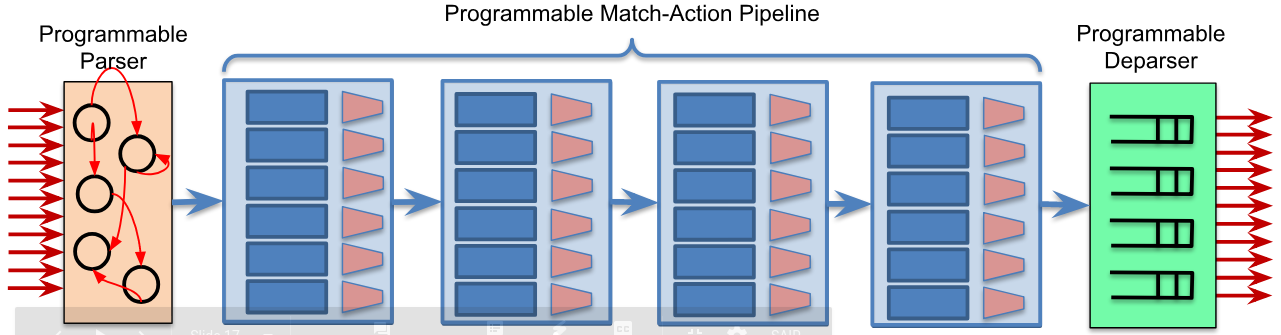
\includegraphics[width=\textwidth]{images/pisa.png}
    \label{fig:pisa-model}
\end{figure}

De forma geral, a linguagem funciona de forma bem direta, onde o programador define
os cabeçalhos que serão utilizados, assim, quando um novo pacote chega para processamento
seus campos são separados em campos individuais de acordo com as regras descritas e são
passados para as tabelas. As tabelas possuem como entrada os campos do cabeçalhos e 
resultados parciais, com essas informações, as tabelas executam diferentes ações,
como remover ou adicionar cabeçalhos, funções aritméticas e mover valores. Após o 
processamento pelas tabelas, as informações são passadas para o deparser, que 
monta os pacotes e transmite de volta para rede \cite{p4LangTutorial}.

\subsubsection{Componentes da linguagem}

A linguagem utiliza um modelo abstrato para redirecionamento de pacotes, que possui
dois tipos de operações, \emph{configure} e \emph{populate}. Durante a operação
de \emph{configure}, o parser é criado, é definida a ordem de estágios nas tabelas
\emph{match+action} e quais os campos do cabeçalhos são processados em cada estágio,
durante a operação de \emph{populate} adicionam e removem entradas nas tabelas
\emph{match+action} construídas durante operação de \emph{configure}. Assim,
durante \emph{configure}, é definido qual protocolo será utilizado e como será
o processamento dos pacotes, e durante \emph{populate} é determinada qual a 
política utilizada nos pacotes \cite{bosshart2014p4}.

A linguagem possui alguns componentes centrais, o primeiro desses componentes 
é o cabeçalho, cada cabeçalho é definido seguindo o nome do campo em conjunto 
com seu tamanho, campos que possui tamanho variável, devem ser definidos com o
tamanho máximo que esse campo pode possuir, um exemplo da definição de cabeçalho
seria:

\lstinputlisting[language=c++, caption={header.p4}]{code/p4-example/header.p4}

Outro componente é o parser, o parser especifica quais campos do cabeçalhos estão
bem definidos e como encontrar esses campos. Os campos extraídos dos cabeçalhos e 
são enviados para tabela de \emph{match+action}, onde será processado e seguirá
para o próximo passo, agindo de maneira semelhante a uma máquina de estados, em 
que as transições são realizadas por valores nos campos do cabeçalho. Um parser
segue a seguinte definição:

\lstinputlisting[language=c++, caption={header.p4}]{code/p4-example/parser.p4}

O parser é iniciado em \texttt{start}, é segue até encontrar um \texttt{stop} ou não
encontrar nenhum match, o que seria um erro \cite{bosshart2014p4}. O parser cria um 
\emph{parsed packet} em que a tabela de \emph{match+action} irá utilizar,
assim, valores que serão utilizados no processamento devem estar contidos nesse
\emph{parsed packet} \cite{p4USITutorial}.

O componente fornecido pela linguagem para o processamento dos pacotes são as tabelas,
de acordo com matches em campos do cabeçalho, esse match  pode ser exato, parcial 
ou ser algum "coringa", são especificados quais as ações serão executadas no
pacote. Utilizando a definição da tabela, o compilador pode decidir quanta memória 
é necessária e qual o tipo de memória necessária \cite{bosshart2014p4}. A
tabela é um componente que aponta qual ação deve ser realizada, assim, não é a 
tabela que executa a ação em si. A definição da tabela segue a seguinte forma:

\lstinputlisting[language=c++, caption={header.p4}]{code/p4-example/table.p4}

Pela definição da tabela pode se notar assim, que a ação é outro componente presente
na linguagem. Com a ação, é possível criar comandos mais complexos para primitivas
presentes no cabeçalho dos pacotes \cite{bosshart2014p4}. Ações funcionam de
maneira imperativa através de suas primitivas, podendo modificar, adicionar ou 
remover campos do cabeçalho, alterar campos dos metadados, realizar operações
que mantém um estado \cite{p4USITutorial}. O exemplo da estrutura de uma ação
é a seguinte:

\lstinputlisting[language=c++, caption={header.p4}]{code/p4-example/action.p4}

Caso uma ação necessite de parâmetros para ser executada, como no exemplo com
\texttt{value} e \texttt{egr\_spec}, esses parâmetros são fornecidos pela tabela em tempo 
de execução \cite{bosshart2014p4}.

O último componente é o controle de programa, utilizando funções, condições e referências
a tabelas, é definido o fluxo de uma tabela para a próxima, assim, o controle de programa
consiste em um programa imperativo que descreve o fluxo entre tabelas \emph{match+action} 
\cite{bosshart2014p4}. Um exemplo de como é o controle do programa: 

\lstinputlisting[language=c++, caption={header.p4}]{code/p4-example/program.p4}

Para a implantação do programa definido em dispositivos de rede, é necessário realizar
a compilação para mapear a descrição que está independente para o alvo em que se deseja
trabalhar. A compilação do controle de programa é realizada em duas etapas, inicialmente
é gerada uma representação intermediaria, onde o programa é representado como grafo de
dependências entre tabelas, que é analisado para verificar dependências entre as tabelas
e verificar quais campos de cabeçalho podem ser processados em paralelo. A segunda etapa
utiliza o grafo resultante da primeira etapa, que é mapeado para utilizar os recursos
específicos do dispositivo alvo em que se vai trabalhar \cite{bosshart2014p4}.

\subsubsection{Ferramentas oferecidas}
Outras ferramentas também são oferecidas pelo P4 Lang Consortium, dentre elas estão o 
\emph{behavioral model}\todo{FEITO use emph para enfatizar texto. deixe $ $ apenas para conteúdo matemático.}, também chamado de \emph{bmv2} e o \emph{p4c-bm}. O \emph{behavioral model} é utilizado 
para executar os programas escritos em P4, oferece também na linha de comando uma interface 
para popular as tabelas inicialmente, se conectando através de um servidor \emph{thrift} e podendo 
assim, por exemplo, definir qual a ação padrão de uma tabela. Através da linha de comando do 
\emph{behavioral model} também é possível configurar como será o \emph{multicast}. Para executar esses 
comandos, é preciso fornecer a representação do programa P4 em formato \emph{JSON}
\footnote{JavaScript Object Notation}, isso pode ser obtido utilizando o \emph{p4c-bm}, que gera a 
representação pronta para ser utilizada no \emph{behavioral model}.

Com a arquitetura e ferramentas definidas, é possível, por exemplo, implementar o roteamento 
de pacotes IPv4. Assim, é possível notar que para implementação do projeto, a utilização da P4
é uma ótima escolha, visto que ela é flexível para criação dos pacotes e campos de cabeçalho
para execução do Paxos, e é possível realizar uma implementação que não fique atada a 
dispositivos de rede específicos.

\subsection{Mininet}
Mininet é um simulador de redes, que executa uma coleção de hosts finais, switches, 
roteadores e links, em uma única máquina. Os programas que utilizam dessa rede, podem enviar
pacotes e estes são processados, de maneira semelhante a rede Ethernet \cite{mininetDocs}.
Desta forma, para o presente projeto, é possível construir a rede utilizando o Mininet, e 
assim ser testada a implementação do Paxos nos dispositivos dessa rede.

Internamente, o Mininet realiza a virtualização encontradas no kernel do Linux, onde é possível
iniciar e escalar mais rápido do que sistemas que emulam a rede utilizando máquinas virtuais
\cite{mininetDocs}. Nesse modelo de virtualização, um único sistema é separado em diversas
partes menores, cada um destes possuindo uma parcela do poder de processamento e links virtuais
\cite{mininetDocs}.

Com a instalação do Mininet, é possível definir topologias de forma rápida e prática, a partir
de um interface pela linha de comando ou utilizando uma API em Python para orquestração da rede.
A partir da linha de comando, é possível executar comandos em nós específicos da rede 
\cite{mininetDocs}. 

\subsubsection{CLI}
Para iniciar a interface do Mininet pela linha de comando, com a topologia
\emph{minimal}, que consiste em 2 processos hosts, 1 processo switch e 1 controlador
básico, basta executar \cite{mininetOrg}:

\begin{minted}{bash}
  $ sudo mn
\end{minted}

Outras opções de topologia podem ser passadas com o argumento \texttt{--topo}. Para se testar a
conectividade entre os hosts, basta executar:

\begin{minted}{bash}
  mininet> h1 ping -c 1 h2
\end{minted}

Para \emph{h1} descobrir o endereço de \emph{h2}, ele realiza um ARP, fazendo com que o evento de 
\texttt{packet\_in} vá para o controlador. O controlador realiza um \emph{broadcast} em todas as portas
com a mensagem de \texttt{packet\_out} no \emph{switch}. Assim, quando \emph{h2} recebe a requisição ARP ele
envia uma resposta, que passa pelo controlador e retorna para \emph{h1}, que agora conhece o endereço
de \emph{h2}. Com \emph{h1} agora possuindo o endereço de \emph{h2}, envia o \emph{echo request} utilizando
protocolo ICMP, e \emph{h2} responde com \emph{echo reply}.

\subsubsection{Python}
Utilizando a API em Python, também é possível definir diferentes topologias para a rede. Um
exemplo simples consiste em uma topologia que possui 2 hosts e 2 switches, distribuídos como
a figura \ref{fig:custom-topology-example}. Para se definir essa topologia, utilizando
Python, fica da seguinte maneira:

\lstinputlisting[language=python,
caption={custom-topology.py}]{code/ninet-example/topo-2sw-2host.py}

Iniciando o Mininet no terminal, indicando qual a topologia utilizada, com o seguinte comando:

\begin{minted}{bash}
  $ sudo mn --custom custom-topology.py --topo custom_topo
\end{minted}

A API em Python possuem três níveis, definidos como API em baixo nível, API em nível médio e API
em alto nível, essa distinção é feita com o intuito de se construir componentes de alto nível
a partir de componentes de baixo nível \cite{mininetDocs}.

Baixo nível consiste de classes para os nós e os links, utilizando instâncias dessas 
classes é possível construir uma rede. Essas classes são \texttt{Host}, \texttt{Switch} e
\texttt{Link} e suas subclasses \cite{mininetDocs}.

O nível médio da API, consiste da classe \texttt{Mininet}, que se trata de um container,
que encapsula a criação de nós e links da rede, assim como a sua configuração \cite{mininetDocs}.

Em alto nível consiste a abstração \texttt{Topo}, para que se possa criar modelos de topologias 
parametrizadas e reutilizáveis, de modo que esses modelos possam ser passados para Mininet
pela linha de comando.

\begin{figure}[ht]
    \caption{Topologia personalizada utilizando Python}
    \centering
    
\includegraphics[width=\textwidth]{images/2sw-2host.png}
    \label{fig:custom-topology-example}
\end{figure}

Visto que a utilização de verdadeiros \emph{switches} e roteadores pode ser caro para simulação do
projeto, podemos utilizar a simulação que o Mininet oferece para resolver esse problema.
Como observado no exemplos, podemos utilizar diferentes topologias, que são criadas e 
executadas de forma prática, assim facilitando nos experimentos.

\section{Trabalhos Correlatos}
Essa seção visa listar trabalhos relacionados com o presente projeto, alguns destes usados
como material de referência para o desenvolvimento, esses trabalhos possuem experimentos
realizados previamente, utilizando ferramentas semelhantes as utilizadas no presente projeto 
e tais trabalhos deixaram áreas para futuras pesquisas sobre o tema.

\subsection{Paxos Made Switch-y}
Trabalho publicado em 2016, realizado por pesquisadores da Università della Svizzera italiana
e Université catholique de Louvain. Neste trabalho, foi realizada uma pesquisa com o intuito
de se realizar a implementação do Paxos para dispositivos de rede utilizando a linguagem
de programação de plano de dados P4, onde os testes para isso foram utilizando o Mininet. 
A pesquisa realiza também uma discussão sobre as linguagens de programação de plano de dados,
em específico a linguagem P4, onde foi relatado que a implementação é uma
implementação não trivial para linguagem, também abordam pontos como tratamento de erros,
dentre outros pontos. Foi realizada também uma discussão sobre protocolos de consenso,
onde os protocolos normalmente só assumem uma conexão ponto-a-ponto, seria interessante a
construção de protocolos que assumem outras propriedades da rede, pois existe um avanço
no hardware utilizado, assim, a performance dos protocolos poderiam ser melhoradas 
\cite{dang2016paxos}.\todo{alem do paxos made switch-y, tem a dissertação e um outro artigo publicado depois.}

%######################### DESENVOLVIMENTO ##################################
\chapter{Desenvolvimento}
O desenvolvimento do projeto seguirá como descrito no cronograma, sendo divido em 
3 fases. Para cada uma das fases realizadas, seguirá uma explicação do que foi realizado,
dos códigos utilizados e uma breve explicação de qual o intuito que se deseja realizar.

O desenvolvimento foi realizado em uma máquina 64 bits utilizando Linux, especificamente a 
distribuição \emph{Arch} com o \emph{kernel 5.1.4-arch1-1-ARCH}.

\section{Reprodução}
Nessa subseção descreverá como se deu a replicação do projeto de \cite{dang2016paxos}, como foi realizada 
a criação do ambiente e quais foram os testes
realizados. O código utilizado no projeto passado pode ser encontrado no \emph{GitHub}
\footnote{https://github.com/usi-systems/p4xos-public}, possuindo os passos que
se deve realizar para execução do projeto e dos testes. Para o presente projeto foi 
criado um repositório contendo todo código, que também pode ser encontrado no \emph{GitHub}
\footnote{https://github.com/jabolina/monography-code}, desta forma ficando aberto
para contribuições e para ser utilizado em outras pesquisas e projetos.

\subsection{Ambiente}
Para execução do projeto, é criada uma máquina virtual que utiliza \emph{Vagrant} para
manutenção, instalação das dependências e pacotes necessários. O sistema operacional
utilizado é o Ubuntu, da imagem \emph{ubuntu/trusty64}, fornecido pela própria
\emph{Vagrant} \cite{ubuntuTrusty}. Para o funcionamento é necessário indicar qual será
o provedor, para o projeto foi utilizado como provedor a \emph{VirtualBox}, onde foi
alocado 2048 \emph{MBs} de memória RAM e 2 núcleos do processador para a máquina
virtual.

As dependências instaladas são descritas no arquivo \emph{Vagrantfile}, nesse caso,
as dependências são descritas em \emph{scripts bash}, que funcionam como forma
de provisão para máquina, podendo ser \emph{scripts} que simples que criam pastas e arquivos
como também para instalação e preparação do ambiente, como é o caso. O primeiro script 
instala o Mininet, utilizando a versão que possui a \emph{tag 2.2.1}, logo após é instalado 
o \emph{POX}, que se trata de um \emph{framework} para comunicação com os \emph{switches} podendo 
utilizar tanto o protocolo \emph{OpenFlow} como \emph{OVSDB} \cite{poxWiki}. Para o \emph{POX} 
é utilizado um \emph{commit} específico. Um segundo script irá instalar as dependências 
relacionadas a P4, a primeira dependência é o \emph{thrift} que é utilizado por
algumas bibliotecas da P4. Em seguida são instalados dos repositórios da própria P4
as dependências \emph{bmv2} e \emph{p4c-bm}, que são relacionadas a maneira de executar programas em P4.
Os programas em P4 são descritos em \emph{JSON} utilizando \emph{p4c-bm}, depois as estruturas são 
carregadas no \emph{bmv2} utilizando a definição do arquivo \emph{JSON}, assim é possível obter o modo
de roteamento desejado. Juntamente com as dependências, é clonado o repositório do projeto, 
com todo código necessário para executar testes.

\subsection{Teste}

Logando dentro da máquina virtual que se montou, é encontrado a implementação do projeto
passado, possuindo uma demonstração para utilização. Com essa demonstração, é possível
inserir valores relacionados a uma chaves e buscar por valores dado uma chave, utilizando
a linha de comando do Mininet é possível simular falhas na rede. Existe também um \emph{script}
para testar inserção e pesquisa de valores, o \emph{script} insere um valor, pesquisa pela chave
associada a esse valor e pesquisa por uma chave não existente.

\begin{figure}[ht]
    \caption{Topologia da demonstração \cite{dang2016paxos}}
    \centering
    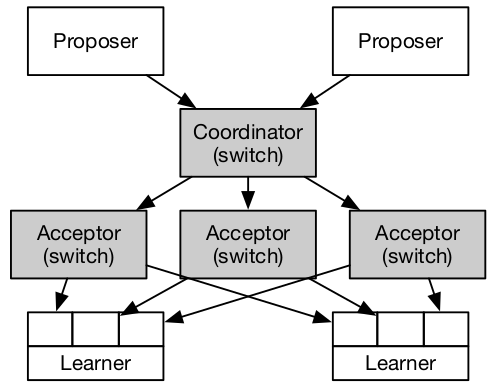
\includegraphics[scale=0.8]{images/arq.png}
    \label{fig:demo-topo}
\end{figure}

Essa demonstração e o projeto segue a topologia descrita por \ref{fig:demo-topo}, em que os
que estão coloridos em branco são executados em servidores.

\subsection{Funcionamento do projeto}
Para iniciar a execução da demonstração, é executado um script em Python, que irá definir a
topologia com o Minininet, que irá utilizar \emph{switches} programados, que executam os \emph{acceptors}
e \emph{coordinator}, com a topologia definida, as tabelas nos \emph{switches} são populadas, definindo
quais os valores utilizados na tabelas para executar o \emph{match} no tipo de mensagem, definindo o
grupo de \emph{multicast}. Após execução do script, será possível realizar requisições no servidor
que foi aberto no \emph{proposer}.

Quando o servidor recebe uma requisição, irá criar um novo pacote e inserir as informações no
cabeçalho para serem transportados, o formato do cabeçalho segue como definido em \ref{cod:p4-header}, 
possuindo o campo definindo o tipo da mensagem, com tamanho de 8 bits, o número da instância com tamanho 16 bits,
um campo definindo o round da instancia e o round em que o voto foi realizado, ambos com tamanho de
8 bits, o campo \texttt{acceptor} contém o identificador do switch com tamanho de 64 bits e o valor do
voto com tamanho de 512 bits.

\lstinputlisting[language=c,caption={Cabeçalho do P4xos}, label={cod:p4-header}]{code/p4xos/explanation/headers.p4}

Assim, o \emph{propopser} irá enviar a requisição, que irá chegar no \emph{coordinator}. O \emph{coordinator} garante que
somente um processo envie uma mensagem para o protocolo para uma dada instância, isso garante 
que o protocolo irá finalizar e impõe uma ordenação nas mensagens, como existe somente um
\emph{coordinator} para identificação e ordenação das mensagens, uma simples sequência crescente pode ser
utilizada. A ação que o \emph{coordinator} deve executar, quando em posse de uma pacote válido do Paxos,
deve ser de definir o tipo de mensagem do protocolo, definir o valor do \texttt{round} como 0, pois
uma nova instância foi iniciada, ler da memória não-volátil qual o número da última instância e atualizar
o valor\cite{dang2016paxos}.

\lstinputlisting[language=c,caption={P4xos coordinator}]{code/p4xos/explanation/coordinator.p4}


Após realizar as ações, o \emph{coordinator} irá realizar um \emph{broadcast} do pacote para todos \emph{acceptors}.
Os \emph{acceptors} que irão assegurar que somente um valor seja escolhido por instância, eles também deve tolerar
mensagens perdidas ou duplicadas. As mensagens que tratadas são do tipo 1A ou 2A, as mensagens do
tipo 1A são utilizadas durante a inicialização do protocolo, enquanto mensagens do tipo 2A são utilizadas
para votação. Em ambos os casos, as ações dos \emph{acceptors} consistem em definir o tipo seguinte da mensagem,
atualizar o valor do \emph{round} na memória não-volátil, armazenar no cabeçalho o valor votado, o número do
round que foi realizado o voto e o identificador do \emph{acceptor} que realizou o voto. Para realizar
essas ações, deve ser verificado de qual \emph{round} pertence a mensagem que chegou para ser processada,
caso o \emph{round} presente no cabeçalho seja menor do que o valor armazenado na memória, o pacote será 
dropado\cite{dang2016paxos}.

\lstinputlisting[language=c,caption={P4xos coordinator}]{code/p4xos/explanation/acceptor.p4}

Após realizado o processamento pelo \emph{switch}, cada um deles realiza um \emph{broadcast} do pacote,
com as alterações, caso existam. Com o \emph{broadcast} realizado, as mensagem chegam aos
\emph{learners}, que são aplicações que estão sendo executadas em servidores \ref{fig:demo-topo}, 
na demo disponível, existem 2 \emph{learners}, que executam a mesma aplicação.

A aplicação executada pelos \emph{learners} ficam realizando um \emph{sniff} na rede, filtrando pacotes
\texttt{UDP} que vierem por uma porta específica, no caso a porta \texttt{34952}. Quando um
pacote é capturado, é realizado um \emph{parse} para ter acesso as campos disponíveis no pacote, dentre
eles o tipo da mensagem, referente ao tipo da mensagem do Paxos. Os \emph{learners} realizam o processamento
de mensagens do tipo \texttt{1B} e \texttt{2B}. Mensagens do tipo \texttt{1B} são salvas no históricos
disponível no \emph{learner} e então são enviadas de volta para rede como mensagem do tipo \texttt{2A}.

Para as mensagens do tipo \texttt{2B}, é verificado se já existe o valor da mensagem no histórico
do \emph{learner} e se já está finalizada, caso a instância já tenha sido finalizada, é retornado o
número de requisição e o valor definido pelo consenso. Caso a instância não tenha sido finalizada,
o novo \emph{acceptor} que votou é adicionado no histórico de votos da instância e assim é verificado
se a maioria de \emph{acceptors} já votaram na instância, para assim ser encerrada e salva na histórico
do \emph{learner}. Quando em posse do valor definido em uma instância, o \emph{learner} irá enviar um pacote de 
volta para o servidor que realizou a requisição, contendo o identificador da requisição e o valor definido.

\section{Extensão}
Está seção irá analisar alguns pontos em que o projeto pode ser melhorado, o porquê de ser um ponto de
melhora e será apresentado de que maneira será realizada essa melhoria.

\subsection{Pontos de melhora}
Os pontos de melhora perceptíveis foram na questão do número de instâncias possíveis de serem executadas,
esse valor é definido pelo campo \texttt{instance} no cabeçalho. o número de instâncias que pode ser 
computado na primeira fase do Paxos é limitado por esse valor, dessa forma, se for utilizado um valor
muito pequeno o consenso será executado por um pequeno período de tempo, mas por ser realizadas operações
utilizando esse valor, caso seja muito grande, pode impactar na performance \cite{dang2016paxos}. 
Quando realizados testes para simular um valor que exceda o valor que os bits conseguem representar 
para o valor da instância, o projeto para e não se consegue obter mais respostas para as requisições.

Pelo arquitetura utilizada para o \emph{switch}, quando ocorre um \emph{overflow} no campo de cabeçalho, assim,
o valor volta pra 0, isso poderia ajudar o algoritmo a seguir computando novas instâncias, mas como
os registradores utilizados estão com valores utilizados previamente, isso impossibilita a continuação
do algoritmo.

A melhora aqui proposta seria a utilização do algoritmo da janela deslizante para manejar as instâncias,
desta forma, poderia ser definido um valor razoável para o número de instâncias, que mesmo após atingir
esse valor continuaria a ser realizado o consenso. Com a implementação da janela deslizante é necessário
se manter atento a alguns problemas que podem surgir. Como lidar caso chegue uma mensagem
de uma instância antiga, e, possivelmente, já encerrada? Como lidar com os registradores que identificam
o número do \emph{round} e de valores de uma instância que precisam ser limpos?

Para o primeiro problema, foi definido que existirão três intervalos possíveis, sendo eles o intervalo
de instâncias ativas e que podem ser executadas imediatamente, o intervalo de instâncias antigas que
estão marcadas para morrer e o intervalo de futuras instâncias. Com a chegada de uma nova mensagem, se o 
número da instância que ela pertence estiver no intervalo de instâncias marcadas para morrer, a mensagem
será ignorada, assim forçando que a instância chegue a um fim. Caso o número da instância estiver no
intervalo de futuras instâncias, a janela irá deslizar 1 casa, em outras palavras, os registradores terão
os valores atualizados com os novos valores dos intervalos, e em seguida, o pacote será enviado de volta 
para o ingresso do \emph{switch}. No último caso, caso o número de instância seja válido,
a execução seguirá seu fluxo normal.

Para limpeza dos registradores que armazenam os valores dos \emph{rounds} e os valores votados, foi implementado
juntamente com o deslizar da janela. Sempre que uma uma instância se inicia e está presente no intervalo de
futuras instâncias, antes da janela deslizar para direita, os registradores presentes na fronteira de 
instâncias marcadas para morrer terão seus valores sobrescritos com o valor 0, assim, o algoritmo poderá
seguir sabendo que quando os registradores forem reutilizado não irá conter nenhum valor que poderá atrapalhar
no desenvolvimento do algoritmo.

\section{Validação}
Esta seção relatará como foi realizada a implementação das melhorias propostas, discutirá como foi realizado
os testes e também de possíveis melhorias que podem ser criadas nessa nova versão.

\subsection{Alterações}
Para as melhorias relatadas, as alterações se concentraram principalmente nos \emph{acceptors}, onde cada um armazena 
em seus registradores os valores dos intervalos das janelas. Com a inserção de novos registradores, foram
realizados alterações nos comandos para popular as tabelas no \emph{switches} e definir quais seriam os comandos padrões
de cada uma delas.

Algumas alterações mínimas foram criadas, como uma campo para marcar se um pacote deve ou não ser descartado no egresso,
para assim não existir a necessidade de chamar uma função de \emph{drop} no mesmo espaço em que se chama funções para o
processamento do pacote, dessa maneira, é necessário somente marcar uma \emph{flag} presente nos metadados do pacote,
caso exista necessidade de descarte.

O funcionamento do projeto segue o mesmo definido anteriormente, onde as alterações agora ocorrem no processamento
do pacote nos \emph{acceptors}, onde são realizadas mais validações para verificar o intervalo da janela em que a instância
está presente.

\subsection{Código}
Referente ao coordenador, não houve alterações em relação a versão anterior, o funcionamento permanece o mesmo.
Quando um novo pacote com os cabeçalhos do tipo \emph{paxos} é aplicada a tabela para recuperar o valor da última instância
processada, é adicionado 1 a esse valor e reescreve esse valor no registrador que mantém o valor da instância, após isso,
o pacote segue para o egresso. Relembrando, a arquitetura utilizada para o experimento é fornecida pela P4 Consortium, é
chamada como \emph{simple switch}, nessa arquitetura, quando o valor é adicionado no número de instância o \emph{overflow} vai para
0, dependendo da arquitetura utilizada, esse \emph{overflow} deve ser tratado de maneira diferente, pois poderia acarretar em
erro no processamento do pacote.

\lstinputlisting[language=c,caption={Registradores adicionados no acceptor},label={cod:changes:register}]{code/p4xos/changes/register.p4}

O próximo passo, é o processamento realizado pelo \emph{acceptor}, e é onde reside a maior parte das alterações realizadas no projeto.
Onde antes existiam 3 registradores, foram adicionados outros 3, que são para armazenar o valor da margem de instâncias marcadas
para morrer, o valor da margem das instâncias válidas e para armazenar a margem das novas instâncias. Todos os registradores
comportam valores que podem ser representados por 16 bits, ou seja, valores no intervalo de 0 até $(2^{16} - 1)$ \ref{cod:changes:register}.

\lstinputlisting[language=c,caption={Tabelas e ações adicionadas no acceptor},label={cod:changes:tables}]{code/p4xos/changes/tables.p4}

Para lidar com os novos registradores, foram adicionadas novas tabelas e ações. Foi adicionada um tabela para lidar com os
valores dos intervalos da janela, com nome \texttt{tbl\_inst} que executa a ação \texttt{read\_instance}, essa ação é executada
sempre que um novo pacote \emph{paxos} válido chega para o processamento, ela é encarregada de ler os valores dos registradores
que armazenam os valores dos intervalos de instâncias marcadas para morrer, de instâncias válidas e de novas instâncias, 
e armazenar esses valores nos metadados do pacote. Outra tabela adicionada foi a \texttt{tbl\_clean\_register}, que executa
a ação \texttt{clean\_register}, esse função irá realizar a limpeza dos registradores sempre que a janela se deslocar, colocando
0 nos registradores de \emph{round}, valores e \emph{vround}. A última tabela adicionada foi a \texttt{tbl\_slide\_window}, que executa a
ação \texttt{slide\_window}, essa ação irá adicionar 1 aos valores da janela e irá reescrever o novo valor nos registradores referentes
a cada um, ao fim irá realizar um \texttt{submit}, visto na linha 26 em \ref{cod:changes:tables}. Essa ação pertence a P4, recebe uma
lista de campos para para ser ressubmetidas ao processamento, mas antes de ir para o ingresso do \emph{switch}, o pacote prossegue o
fluxo normal até o egresso, ou seja, caso o pacote esteja marcado para descarte a ressubmissão não será executada, isso ajuda
no processamento, pois caso existissem mais casos para se tratar, o pacote segue o fluxo normal de execução, ativando
tabelas e ações.

Essas adições são utilizadas pelo \emph{acceptor} no ingresso, para o processamento de pacote válido do \emph{paxos}. Inicialmente se
aplica as tabelas \texttt{tbl\_inst} e \texttt{tbl\_rnd}, para recuperar dos registradores os intervalos da janela e o valor 
do round. Com esses valores presentes nos metadados do pacote, verifica se o último round salvo em registrador é menor
ou igual ao round do atual pacote, caso o round seja válido, o processamento prossegue, onde então será verificado o intervalo
da atual instância. Para explicar os diferentes casos, a imagem \ref{fig:window-intervals} será utilizada como referência.

\begin{figure}[ht]
    \caption{Intervalos da janela}
    \centering
    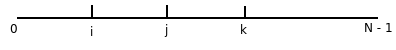
\includegraphics[scale=0.8]{images/windowOk.png}
    \label{fig:window-intervals}
\end{figure}

\todo{FEITO. N ou N-1? O tamanho da janela total é N+1?}

Com a janela dividida em três intervalos, existem 3 cenários diferentes que uma nova instância pode se encontrar durante o
processamento. O primeiro e mais simples de ser tratado, é quando uma nova instância de número \texttt{X} chega para
o processamento, e X possui valor $j \leq x < k$, ou seja, o número está presente no intervalo de instâncias válidas. 
Desta forma, o pacote prosseguirá o fluxo normal de processamento.

Existe também a possibilidade de um pacote se atrasar e chegar para o \emph{proposer} um pacote de uma instância de número
\texttt{X} com valor $i \leq X < j$, ou até mesmo $X < i$, isso significa que o número está no intervalo de instâncias
marcadas para morrer. Instâncias que residem nesse intervalos, terão os pacotes marcados para descarte, assim, quando
chegarem no egresso os pacotes serão dropados.
O terceiro e último cenário para o valor de uma instância \texttt{X} é o valor $k \leq X$, ou seja, a janela deve deslizar,
assim primeiramente serão limpos os registradores de índice \texttt{i}, em seguida serão atualizado os valores de
intervalos nos registradores e por fim, executa o \texttt{resubmit} do pacote.

Com o deslizamento da janela, chegaram o ponto que deve existir um restart dos intervalos, desta maneira, é possível
imaginar a janela como um anel, onde numa janela de tamanho $N$, o primeiro número logo após o $N$ é o 0. Pela 
existência de 3 intervalos, existirão também 3 cenários existentes. O mais simples é o quando a janela é iniciada,
e segue deslizando da esquerda para direito, e, utilizando \ref{fig:window-intervals} como referência, os intervalos
se mantém com $i < j < k$, que é exatamente o caso demonstrado pela figura. No decorrer do algoritmo, o primeiro intervalo
que precisará ser resetado é o de novas instâncias, com esse reset, existe um novo cenário, o caso em que $k < i < j$.
O próximo e último caso, ocorre quando ocorre ambos o reset do valor $k$ e em seguida do valor $j$, tendo assim,
os intervalos da janela como $j < k < i$. Quando o reset do último intervalo ocorre, se retorna para o estado normal,
tendo os valores como $i < j < k$.

\begin{algorithm}[H]
\label{alg:slide-window}
\caption{Processamento de pacote de acordo com intervalos}
\SetAlgoLined
\Inicio{
$X$ = número da instância

$i$ = intervalo marcado para morrer\\
$j$ = intervalo válido\\
$k$ = intervalo novas instâncias

\Se{i < j < k}{
    \Se{$(i < X) \land (j \leq X) \land (X < k)$}{
        processar mensagem;
    }
    
    \SenaoSe{$(k \leq X) \land (i < k)$}{
        limpar registradores;\\
        resubmit;
    }
}
\SenaoSe{$k < i < j$}{
    \Se{$(j \leq X) \lor (X < k)$}{
        processar mensagem;
    }
    \SenaoSe{$(k \leq X) \land (X < i)$}{
        limpar registradores;\\
        resubmit;
    }
}
\SenaoSe{$j < k < i$}{
    \Se{$(j \leq X) \land (X < k)$}{
        processar mensagem;
    }
    \SenaoSe{$(k \leq X) \land (X < i)$}{
        limpar registradores;\\
        resubmit;
    }
}
}
\end{algorithm}

Para conseguir tratar os possíveis cenários que podem surgir, foi implementado no ingresso do \emph{switch} o algoritmo
apresentado em \ref{alg:slide-window}. Observando pelo algoritmo, todas instâncias que estiverem presentes no intervalo de 
instâncias marcadas para morrer, ou se o \emph{round} da instância não for válido, não passarão em nenhuma das verificações, esses 
pacotes serão descartados no egresso do \emph{switch}.


\subsection{Experimento}
Para realizar o experimento, foi reutilizada a estrutura do projeto passado, tanto a estrutura da rede como das 
aplicações utilizadas para teste. A estrutura da rede utiliza 4 \emph{switches} e 4 \emph{hosts},
dentre os \emph{switches}, 1 foi designado para ser o coordenador e os outros 3 foram designados como \emph{acceptors}.
Para os \emph{hosts}, 1 deles executa um servidor aberto na porta 8080, que irá receber requisições de leitura
e escrita em um dicionário, outros 2 \emph{hosts} executam a função de \emph{learners} e 1 dos \emph{hosts} é executado
somente para realizar requisições no servidor \ref{fig:demo-topo}.

Para execução da demonstração, foi utilizada a máquina virtual, a mesma utilizada para replicação do projeto
passado \cite{dang2016paxos}. Com a rede criada, é aberto um terminal no \emph{host} 4, e, a partir dele,
é executado um \emph{script} para realizar requisições no servidor presente no \emph{host} 1, são realizadas
3 requisições diferentes por iteração do \emph{loop}. Realizada uma requisição para inserção de um novo valor juntamente
com uma nova chave na memória da aplicação sendo executada nos \emph{hosts}, em seguida é realizada uma requisição para 
leitura passando a mesma chave inserida anteriormente e por fim uma requisição para uma chave que não existe.

Para experimentação foram criados alguns cenários, para testar como a nova implementação se sairia. A primeira, e mais simples
foi a de simplesmente iniciar a demonstração e as requisições a partir do \emph{host} 4, acompanhando os \emph{logs} dos
\emph{learners} presentes nos \emph{hosts} 2 e 3 é possível verificar o número de instância aumentando e verificando que 
o valor só é retornado quando o consenso entre os 3 \emph{acceptors} é atingido. Acompanhando também o \emph{log} dos
\emph{switches} é possível acompanhar o fluxo que o pacote realiza dentro do \emph{switch}, das leituras/escritas de registradores,
comparações realizadas, do ingresso até o egresso. Nesse cenário, a execução acontece normalmente.

Outro cenário criado foi em que o número da instância se inicia em um valor \texttt{X}, que reside no intervalo de novas instâncias,
assim, o funcionamento esperado seria o de que a janela deslizasse de 1 em 1, até o número de instância \texttt{X} pertencer ao intervalo
de instâncias aceitas. Quando iniciado o experimento, para primeira requisição a resposta na é obtida de imediato, dependendo do valor de
\texttt{X} escolhido, pode demorar um tempo, após a primeira resposta ser obtida, as próximas são obtidas uma após a outra, sem muita 
demora da requisição. Acompanhando esse início pelo \emph{log} dos \emph{switches}, é possível ver os registradores sendo limpos,
a janela deslizando e o pacote sendo ressubmetido.

O último cenário criado, foi para verificar a virada da janela. Acompanhando pelo \emph{log} do \emph{switch}, é possível
verificar os valores sendo lidos pelos registradores realizam a virada de N para 0 e as requisições seguem normalmente.
Com a virada, os valores dos antigos \emph{rounds} não influenciaram nas novas instâncias, verificando também que as limpezas
no deslizar da janela também funcionaram. Na implementação utilizada, foi aproveitado o fator da arquitetura do \emph{switch},
em que nos casos que se ocorre um \emph{overflow} no número, ele vai para 0.

\subsection{Melhorias}
No presente, um dos principais pontos que podem ser realizado uma melhoria seria em relação a implementação do \emph{learner}
também em um dispositivo de rede, deixando a implementação nos \emph{hosts} somente como aplicações que vão ser notificadas
ao fim do consenso pelo próprio \emph{learner}.

Durante o desenvolvimento, foi observado que após um longo período de execução, os \emph{switches} param completamente o
processamento de novos pacotes vindo dos \emph{proposers}, monitorando as interfaces de rede nos \emph{hosts}, foi possível 
verificar que o tráfego parava totalmente. Monitorando os \emph{switches} pelos \emph{logs} foi possível observar que durante a
computação das instâncias, assim como visto pelo código, que alguns pacotes são marcados para descarte. Com esse descarte, como a requisição
não obtêm nenhum retorno, o processamento para, só retornando quando é realizado um \emph{ping} entre os \emph{hosts}.
Existem algumas opções que podem ser implementadas para realizar esse tratamento, uma das opções seria o \emph{switch}
responder a origem da requisição com uma confirmação negativa, outra possível solução seria a criação de um temporizador para
a requisição, após o temporizador exceder um tempo determinado o \emph{proposer} envia novamente sua proposta.

\subsection{Discussão}
Esse seção discorrerá sobre a linguagem P4, novos horizontes que podem surgir com as opções que a linguagem oferece e juntamente
irá utilizar exemplos do presente trabalho e sobre as dificuldades encontradas na implementação. Com a possibilidade de programar
\emph{switches}, como Tofino da Barefoot Networks \cite{tofinoSwitch}, são abertas novas possibilidades para os dispositivos de redes,
uma das possibilidades seria a implementação de parte da lógica do sistema, que antes poderia ser executada somente em servidores, como
exemplo, o presente trabalho com a implementação do Paxos.

Com a utilização da linguagem P4, é encontrado um paradigma diferente dos paradigmas convencionais, como imperativo ou orientado a objetos,
é enfrentado uma programação utilizando a abstração de tabelas \emph{match+action}, sem a possibilidade de iterações e ações em baixo
nível. Com a abstração, não possui uma chamada para uma ação diretamente, sendo necessário ativar uma tabela, para assim uma das ações
disponíveis na tabela ser executada. Esse mecanismo pode ser visto claramente na implementação do \emph{learner} do presente trabalho
\ref{cod:acceptor}, onde, por exemplo, para realizar a comparação se o \emph{round} é válido, é necessário invocar a tabela dos \emph{rounds},
que irá ativar a ação para ler os registradores, quando a ação é executada, os valores dos registradores são lidos para os metadados, após
esse processo, a comparação pode ser realizada.

A maior dificuldade encontrada no presente foi encontrar uma maneira para representação das janelas e seu funcionamento. Como a linguagem
não oferece uma maneira de iterar, foi necessário a utilização do reingresso no \emph{switch} para realizar o deslizar da janela, aproveitando
esse funcionamento, foi inserido juntamente o funcionamento para limpeza dos registradores utilizados. Como se trata de um \emph{switch}, caso
exista uma computação muito complexa, pode ser notado na rede um atraso nas respostas das requisições, desta forma, mesmo performance
de execução não sendo o foco no presente projeto, é necessário se manter atento a esses pontos.

A implementação do Paxos, não é uma implementação trivial de ser realizada e a implementação em P4 é possível obter uma visão clara
do funcionamento da P4 e da programação utilizando tabelas, outra visão, é voltada para uma nova maneira de definir protocolos. A área
de protocolos de replicação já é bem madura, mas ainda poucas foram as pesquisas voltadas para protocolos que se aproveitam do comportamento
da rede \cite{dang2016paxos}. Como a possibilidade de programação dos dispositivos de rede, é possível dar um passo adiante nas 
definições de novos protocolos, voltadas para execução nesses dispositivos, visando, por exemplo, protocolos com baixa latência
de execução.


%######################### CONCLUSÃO ##################################
\chapter{Conclusão}
Neste trabalho foi realizada a replicação e implementação de melhorias em um trabalho prévio \cite{dang2016paxos} utilizando
a linguagem de programação P4. Visto que em um sistema de consenso, o número de instâncias a ser executadas é indefinido, foi realizada
a melhoria para o tratamento das instâncias onde antes não havia. Com essa melhoria, conceitualmente, é possível executar
quantas instâncias for necessárias, existindo também o tratamento para valores definidos escritos em registradores por instâncias
antigas não influenciem nas novas instâncias computadas.

Previamente, não existia tratamento paras os valores das instâncias já computadas, e existia um limite definido pelo registrador
que armazena o número da instância, que possui tamanhos de 16 bits, podendo armazenar até $2^{16}$. Como o tamanho da janela pode
ser definido, pode existir um tamanho ótimo, que garante mais processamento é um pequeno número de reingressos dos pacotes para
deslizar a janela. Com a flexibilidade de escolher o tamanho da janela, é possível definir um tamanho, de modo que durante a execução,
os intervalos das janelas se sobreponham, impossibilitando a execução corretamente.

Com o presente trabalho, foi visto que com a possibilidade de programação em dispositivos de redes, é possível executar um algoritmo
de consenso nos próprios dispositivos da rede. Onde foi realizada a extensão em um projeto passado e adicionados métodos para execução
de diversas um número indefinido de instâncias. 

\bibliography{references}

\begin{apendicesenv}
\partapendices
\chapter{Implementação}

Implementação utilizada no projeto, possuindo códigos em P4, projeto completo também está disponível no GitHub.
\footnote{https://github.com/jabolina/monography-code}

\subsection{Coordinator}
\lstinputlisting[language=c,caption={Coordinator em P4},label={cod:coordinator}]{code/extra/coordinator.p4}

\subsection{Acceptor}
\lstinputlisting[language=C++,caption={Acceptor em P4},label={cod:acceptor}]{code/extra/acceptor.p4}

\end{apendicesenv}

\end{document}

